\documentclass[12pt, a4paper]{report}
\usepackage{svg}
\usepackage{lipsum}  
\usepackage{url}
\usepackage{hyperref} 
\usepackage{float}
\usepackage{graphicx}
\usepackage{tikz}
\usepackage{amsmath}
\usepackage{enumitem}

\usepackage{booktabs}
\usepackage{longtable}
\usepackage{tabu}
\usepackage{listings}
\usepackage{tcolorbox}
\usepackage{listings}

\parindent=0pt
\parskip=6pt plus 2pt minus 1pt

\usetikzlibrary {positioning} 
\usetikzlibrary{arrows.meta, quotes}

\graphicspath{{figures/}}

\pagenumbering{arabic}
\title{Bipedal Walking - Reinforcement Learning}
\author{Roberto Figueiredo}
\date{April 2022}


\begin{document}
\begin{titlepage}
    \maketitle 
    \thispagestyle{empty}
\end{titlepage}


\begin{abstract}
 
    This report covers the attempt to develop a bipedal walking pattern using reinforcement learning. 
 
    This project developed a series of experiments progressing from a testing ground using the CartPole environment to a 2D walker and implementation of OpenAI Gym on the RoboCup Team, Bold Hearts, ROS2 environment enabling training for any reinforcement learning task.
    The experiments cover the testing of two different learning implementations and hyperparameter tuning.
    
    
    Although the objective of walking could not be achieved in the target time frame with the limited resources available, the documentation covers the problems found along with how this difficulties were overcome. The implementation chapter will cover how each of the stages was developed, with coding examples for each of the main components.
   
    The results and findings of the experiment will be explored and an attempt to understand what could be changed to achieve achieving the desired outcome.

\end{abstract} 

\section*{Acknowledgement}
\lipsum[1-1]


\pagebreak
\tableofcontents
\pagebreak



\section{Introduction}
Robotic locomotion has, until a few years ago, been focused on wheel-based movement. 
Although it is very stable and easy to implement, it lacks flexibility, the ability to move on uneven, unpredictable terrain and overcome obstacles such as stairs.
\par As a RoboCup team Bold Hearts member, which competes in the humanoid soccer league, our robots must walk, a recurring problem due to rule changes. 
As the objective of RoboCup is to achieve a realistic environment, competition rules change regularly. 
Changes in rules involve field changes, such as moving from flat ground to synthetic grass, enforcing that teams develop walking algorithms that can adapt to more variable environments. 
Rule changes also affect the robots, including their height, types of sensors and others. 
Changes in the robot's structure lead to the need to readapt the walking algorithms as they are dependent on these variables. 
These changes are time-consuming, and walking algorithms are a complex task requiring much effort from the team.
\subsection{Intro to the project}


\chapter{Background Research}
This chapter introduces key background research necessary to understand reinforcement learning and the decisions made. It will cover reinforcement learning, the Markov Decision Process, the Bellman equation, learning algorithms, training frameworks, previous implementations and logging platforms.

\section{Reinforcement Learning}
Reinforcement learning is one of the main machine learning paradigms, alongside supervised learning and unsupervised learning. 
Reinforcement learning aims to map states to actions while maximising a reward signal. In some cases, actions may affect not only the present but future situations. 
To learn how to map the states to actions, the agent must try them. These characteristics, trial-and-error and delayed reward, are the most distinguishable features of reinforcement learning.

The agent must be able to perform actions affecting the environment followed by a perception. This perception should indicate to what state the robot has transitioned and the reward signal associated with the result of the action taken given the previous state. This interaction is summarised in the following figure.

\begin{figure}[H]
 \centering
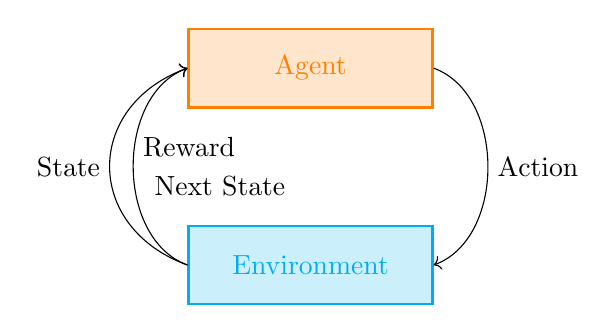
\begin{tikzpicture}[every node/.style=draw]
 \node[rectangle, 
 draw, 
 thick,
 minimum width = 3.1cm,
 minimum height = 1cm,
 color=cyan,
 fill=cyan!20] (A) at (0,0) {Environment};
 \node[rectangle, 
 draw, 
 thick,
 minimum width = 3.1cm,
 minimum height = 1cm,
 color=orange,
 fill=orange!20,
 ] (B) at (0,2.5) {Agent};

 \draw [->] (A.west) to [bend left=70] node [midway,right, draw=none, yshift=+2.5mm]{Reward} node[midway, yshift=-2.5mm,xshift=+11mm,draw=none]{Next State }(B.west);
 \draw [->] (A.west) to [bend left=70, min distance=1.4cm] node [midway,left, draw=none]{State} (B.west);
 \draw [->] (B.east) to [bend left=70] node [midway,right, draw=none]{Action} (A.east);
\end{tikzpicture}
\caption{Reinforcement learning model.}
\end{figure}
One unique challenge in reinforcement learning is balancing exploration and exploitation.
To succeed in a task, the agent must exploit actions that, through experience, have yielded the most rewards, although, 
to have experience and perform better in the future, the agent must explore new actions. 
The dilemma is that neither exploration nor exploitation can be pursued exclusively without failing at the task
\cite{reinforcement_learning}

 \subsection{Markov Decision Process}
 Reinforcement learning can be described using the Markov Decision Process(MDP). MDP is the final summary concept of the individual elements:
 \begin{itemize}
 \item The Markov Property 
 \item The Markov Decision Chain
 \item The Markov Reward Process
 \end{itemize}
 \subsubsection*{Markov Property}
 This means that the transition to state $t_{+1}$ from state {t} is independent of the past, meaning that our current state already captures all the relevant information from the past.
 Defined by the following equation:

 \begingroup
 \Large
 \begin{equation*}
 P(S_{t+1}|S_t) = P(S_{t+1}|S_1,...,S_t)
 \end{equation*}
 \endgroup
 \subsubsection*{Markov Decision Chain}
 A Markov chain is a mathematical system that experiences transitions from one state to another according to certain probabilistic rules. 
 The defining characteristic of a Markov chain is that no matter how the process arrives at its present state, the possible future states are fixed. 
 In other words, the probability of transitioning to any particular state is dependent solely on the current state.
 \begin{figure}[H]
 \centering
 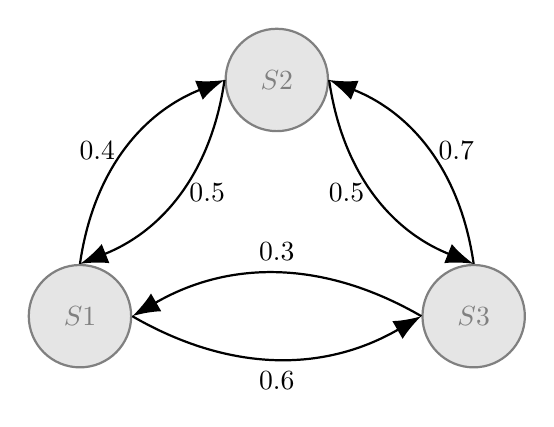
\begin{tikzpicture}[every node/.style=draw]
 \node[circle, 
 draw, 
 thick,
 minimum width = 1.3cm,
 color=gray,
 fill=gray!20] (1) at (0,0) {$S1$};
 \node[circle, 
 draw, 
 thick,
 minimum width = 1.3cm,
 color=gray,
 fill=gray!20] (2) at (2.5,3) {$S2$};

 \node[circle, 
 draw, 
 thick,
 minimum width = 1.3cm,
 color=gray,
 fill=gray!20] (3) at (5,0) {$S3$};

 \draw [->, thick, -{Latex[length=3.5mm]}] (1.north) to [bend left=30] node [midway,left, draw=none]{0.4} (2.west);
 \draw [->, thick, -{Latex[length=3.5mm]}] (1.east) to [bend right=30] node [midway,yshift=-8 ,draw=none]{0.6} (3.west);
 \draw [<-, thick, -{Latex[length=3.5mm]}] (3.west) to [bend right=30] node [midway,yshift=8 ,draw=none]{0.3} (1.east);
 \draw [<-, thick, -{Latex[length=3.5mm]}] (3.north) to [bend right=30] node [midway,right ,draw=none]{0.7} (2.east);
 \draw [->, thick, -{Latex[length=3.5mm]}] (2.east) to [bend right=30] node [midway,left,draw=none]{0.5} (3.north);
 \draw [<-, thick, -{Latex[length=3.5mm]}] (2.west) to [bend left=30] node [midway,right, draw=none]{0.5} (1.north);


 \end{tikzpicture}
 \caption{Example of a Markov Decision Chain.}
 \end{figure}

 As can be observed by the example Markov Decision Chain, the transition probabilities are fixed and are only dependent on the current state, this is the Markov property.

 \begingroup
 \Large
 \begin{equation*}
 P(S_{t+1}|S_t)
 \end{equation*}
 \endgroup

 Definition of the probability of transitioning to any particular state given the current state.


 \subsubsection*{Markov Reward Process}
 As it suggests, the Markov Reward Process is a Markov process with the difference that it includes a reward system that indicates how much reward is accumulated through a particular sequence.
 An additional factor is applied, the \textbf{discount factor $\gamma$} that indicates how much the future reward is discounted. if $\gamma = 0$ 
 then the agent will only consider the immediate reward, if $\gamma = 1$ then the agent will consider all subsequent rewards. 
 In practice, these extreme values are ineffective, and $\gamma$ is usually set to values between 0.9 and 0.99

 \subsection{Bellman equation}
 As the agent moves through the Markov decision chain, one problem develops, how to choose the path that maximises future rewards from the current point onwards. 
 
 To solve this problem, a recursive equation is used, the Bellman equation.
 
 $V(s) = max_a (R(s,a)+\gamma V(s')) $ 
 
 The Bellman equation sums to the present reward the discount factor multiplied by the best next value output by the value function.

 The optimal value function $V^(s)$ maximises the expected reward. To achieve this, the Bellman equation is solved by iteratively updating the value function until $V^(s)$ is reached.

 % Q values are calculated using the Bellman equation, the Bellman equation takes the present reward and sums to it the discount factor multiplied by the best next q value of the combination of the next action and state

\section{Learning Algorithms}
One of the main decisions in implementing a reinforcement learning algorithm is the learning algorithm, to understand the algorithm decision its important to understand how this differ.
\begin{figure}[H]
\centering
\includegraphics[width=1\textwidth]{rl_algorightms.eps}
\caption{A non-exhaustive, but useful taxonomy of algorithms in modern RL from OpenAI\cite{openai_rl}.}
\label{fig:rl_algorightms}
\end{figure}

The first major split in RL algorithms is whether it is model-free or model-based. Model-based algorithms use a model of the environment, which is capable of mimicking its behaviour, this allows inferences to be made about how the environment will behave given an action and what the next reward will be. This reinforcement learning method is inadequate for the current problem due to the high complexity of the environment in which the agent is interacting, making it impossible to model it.

The second decision is between \textbf{policy optimization} and \textbf{Q-Learning}. 
While both approaches have similar concepts and are driven by MDP, they are internally different. 

In Q-learning, the goal is to determine a single action from a set of discrete actions by finding the action with the highest Q-value. While in policy optimisation, the goal is to learn a map from state to action, this can be stochastic and, as opposed to Q-Learning, works in continuous action spaces.

Q-Learning was a better fit for the problem in study as the action space was discretised. Apart from the action space, the Implementation of Q-learning is simpler and more common.

The algorithm decision was set on Deep Q-Network (DQN). The main difference between DQN and Q-Learning is that DQN implements a neural network replacing the Q-table. This is a benefit due to the complexity of the environment and the total number of possible states. Using standard Q-learning would require a very large q-table, which is a huge memory and computational burden.

\section{Training Framework}
Followed by the new advances in RL, there was a growing need for a common benchmarking framework that would allow for comparing algorithms and implementations.

The OpenAI team released Gym to enable this, by providing an accessible API and standardised environments. Gym is now the most widely used tool in RL research, it has a large community and documentation and a growing number of environments\cite{gym}.

Gym was chosen as the framework to standardise the implementation which allows for an easier understanding and comparison, beyond this, the Gym also facilitates the implementation by using all the pre-built functions\cite{openai}.

\section{Previous Implementations}
To develop this project it was important first to study previous implementations, what problems were faced and the reasoning behind their decisions, 
this brought light to many problems and details of implementing reinforcement learning, especially for walking.

One important implementation was the \textbf{Deep Q-Learning for Humanoid Walking}\cite{atlas_rl}, an implementation of reinforcement walking on the Atlas platform.
This implementation highlights some of the general pre-conceptions regarding the reward system and how to handle the complexity of controlling all the joints simultaneously.
%TODO: expand more explored implementations

\section{Logging and Reproducibility}
One of the most important aspects of machine learning and reinforcement learning is data logging and reproducibility. 
This project required extensive testing of hyperparameters and reward systems. 
To understand the results and their correlation with the variables in testing as well as being able to reproduce them, it is important to log all the hyperparameters and results.\linebreak
\textbf{Requirements for logging:}
\begin{itemize}[leftmargin=+0.5in]
 \item Hyperparameters
 \item Performance metrics
 \item Code
 \item Models
 \item Renderings
\end{itemize}
From previous experiences with machine learning and logging platforms, MLflow was the first option analysed. Although Weights \& Biases (WandB) was the chosen platform, WandB offered a hosted version option compared to MLflow. 
WandB also integrates with Keras allowing for a seamless implementation. WandB fills all the requirements and allows for a comparison of the renderings and performance results between runs.


\chapter{Design}
This chapter will be split into two main sections, development structure and environment definition, the first will define how the project will be developed and explain each stage. 
The second section, will define the design for each of the environments used in the development.
\section{Development Structure}
Due to the project's complexity, a development structure has been put in place. This includes multiple steps of increasing complexity and realism. The increasing complexity allows for detecting problems at earlier, simpler stages, making the transition and understanding the problems more manageable.
\subsection{CartPole}
CartPole is a classic exercise of reinforcement learning, it consists in balancing a pole in a cart moving on a horizontal plane by applying a force on the right or left side of the cart, making it move in the opposite direction. 

The CartPole environment allows for implementing and testing the reinforcement learning algorithm, different implementations, and its comparison. At this stage, it is also used to implement the logging and reproducibility interface.

\subsection{2D Walker}
At this stage, the complexity of the environment increases as the environment starts to approximate the target problem. Although, this stage eliminates some of the complexity, such as using a more complex 3D environment and implementing the training with the robot control interface.
This allows for the implementation of a neural network, a learning algorithm capable of handling multiple simultaneous outputs as it is required to control all the joints of the robot and understand how to calculate the best action efficiently.

To achieve this, it is necessary to develop a custom 2D environment of a simplified humanoid in order to train a walking behaviour.
New challenges from this stage, such as implementing a custom reward system, rendering and step functions, are essential steps to transition to 3D simulation.

\subsection{3D Walker}
The final stage of the project is the implementation of a 3D simulated robot. This is the combination of the previous stage with extra complexity, not only due to the inherited complexity of a higher dimensional world but because this should be able to integrate with the real robot from the Bold Hearts team and therefore use its control interface.
Robot simulation is the primary platform for developing software for robotics; it has many benefits, developing software and testing it directly on a real robot can be a very slow process and can even break the robot.

3D simulation brings new challenges, such as a larger range of motion and more joints to control, along with a more complex environment, requiring more processing power and more time to solve the problem. 
Along with this, it requires a more complex reward system as a new dimension poses new problems.

\section{Environment Definition}
One of the main reasons for using OpenAI Gym in this project is the ability to standardize the environments.
In this section, each Gym environment will be described.

\subsection{CartPole}
The CartPole environment is a very simple exercise, consisting of a pole in a cart moving on a horizontal plane. The objective is to balance this pole by applying a force on the right or left side of the cart, making it move in the opposite direction.
\cite{cartpole}

\begin{figure}[H]
 \centering
 \includegraphics[scale=0.24]{CartPole}
 \caption{Rendered CartPole Environment - OpenAI Gym}
\end{figure}

CartPole Environment definition:
\begin{itemize}
 \item \textbf{Observation Space}
 \begin{table}[H]
 \caption{Observation Space for the CartPole environment}
 \centering
 \begin{tabular}{|l|l|l|l|}
 \hline
 Num & Observation & Min & Max \\ \hline
 0 & Cart Position & -4.8 & +4.8 \\ \hline
 1 & Cart Velocity & -Inf & +Inf \\ \hline
 2 & Pole Angle & -24° & +24° \\ \hline
 3 & Pole Angular Velocity & -Inf & +Inf \\ \hline
 \end{tabular}
 \end{table}
 \item \textbf{Action Space} 
 \begin{table}[H]
 \caption{Action Space for the CartPole environment}
 \centering
 \begin{tabular}{|l|l|}
 \hline
 Num & Action \\ \hline
 0 & Push cart to the left \\ \hline
 1 & Push cart to the right \\ \hline
 \end{tabular}
 \end{table}
 \item \textbf{Reward:} In the CartPole environment the reward is attributed per timestep survived, being awarded 1 point per timestep.
 \end{itemize} 

\subsection{2D Walker}
The 2D environment requires a 2D Humanoid, this has been defined with 8 different joints, 2 in the shoulder, 2 in the hips, 2 in the knees and 2 for the ankles.
\begin{figure}[H]
 \centering
 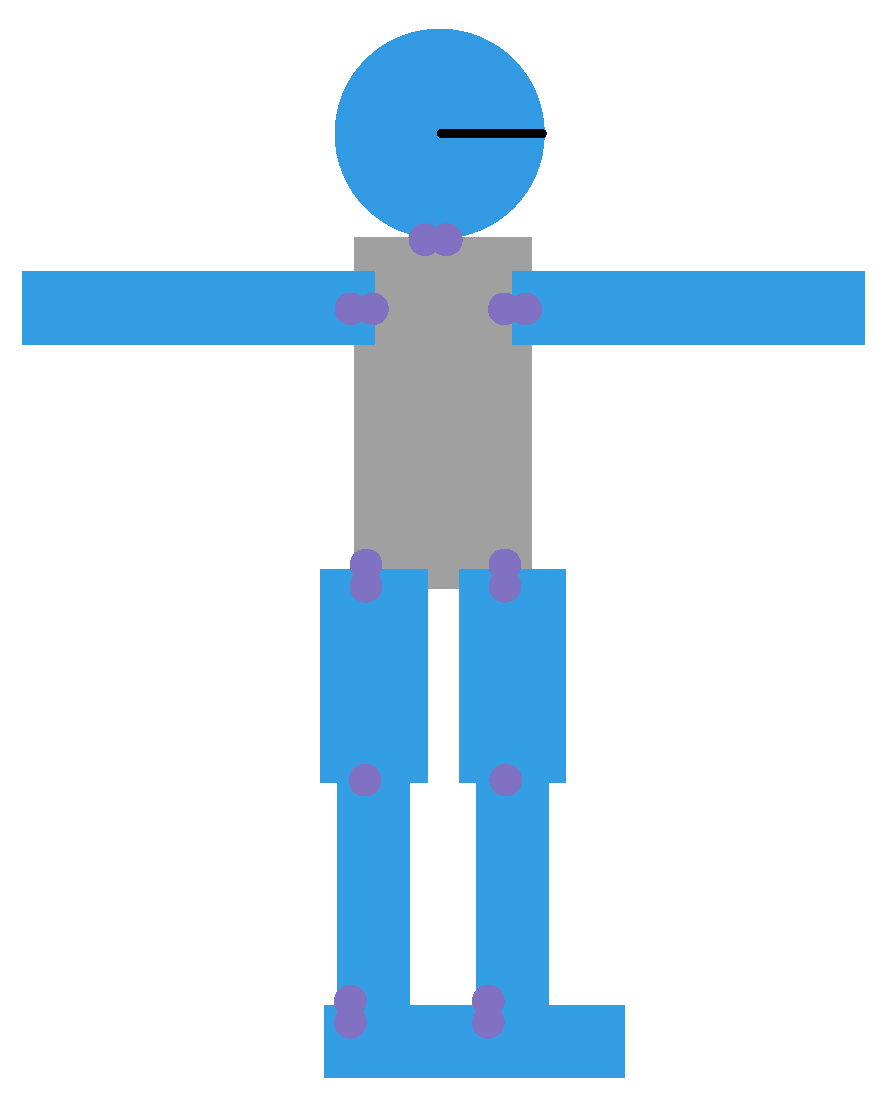
\includegraphics[scale=0.25]{humanoid-2d}
 \caption{Representation of 2D humanoid}
\end{figure}

Environment definition:
\begin{itemize}
 \item \textbf{Observation Space:} The Observation Space is a vector of size 8, containing the angles for each of the 8 joints of the humanoid.
 \begin{table}[H]
 \caption{Observation Space for the 2D Walker environment}
 \centering
 \begin{tabular}{|l|l|l|}
 \hline
 Observation & Min & Max \\ \hline
 Joint Position & -20° & +20° \\ \hline

 \end{tabular}
 \end{table}

 \item \textbf{Action Space:} 
 \begin{table}[H]
 \caption{Action Space for the 2D Walker environment}
 \centering
 \begin{tabular}{|l|l|}
 \hline
 Num & Action \\ \hline
 0 & Move the joint counterclockwise \\ \hline
 1 & Maintain joint position \\ \hline
 2 & Move the joint clockwise \\ \hline
 \end{tabular}
 \end{table}
 \item \textbf{Reward:} 
 \begin{table}[H]
 \caption{Reward system for the 2D Walker environment}
 \centering
 \begin{tabular}{|l|l|}
 \hline
 Action & Points \\ \hline
 Moves Back & 8 \\ \hline
 Stays in Place & 9 \\ \hline
 Moves Forward & 10 \\ \hline
 Loses contact with the ground & cumulative -2 \\ \hline
 Reaches target & 16 \\ \hline
 Falls & 0 \\ \hline
 \end{tabular}
 \end{table}
 
\end{itemize}
The reward is calculated at each timestep, given a threshold $\theta$, the position of the robot is compared to the last position and calculated the offset. If the robot loses contact with the ground with both feet, the reward is subtracted 2 points.
\subsection{3D Walker}
In the 3D environment, the robot needs to simulate the one used by the Bold Hearts team, given that the team already uses a simulator, gazebo, this will be used to interact with the robot given that it provides ROS2 integration.
\begin{figure}[H]
 \centering
 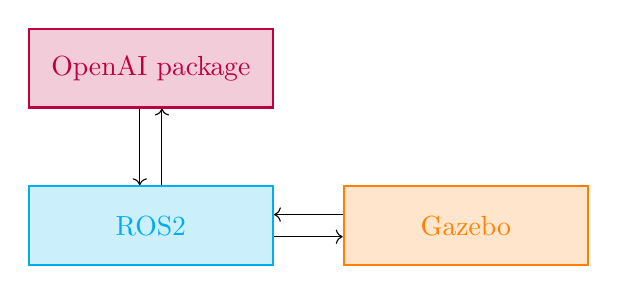
\begin{tikzpicture}[every node/.style=draw]
 \node[rectangle, 
 draw, 
 thick,
 minimum width = 3.1cm,
 minimum height = 1cm,
 color=cyan,
 fill=cyan!20] (A) at (0,0) {ROS2};
 \node[rectangle, 
 draw, 
 thick,
 minimum width = 3.1cm,
 minimum height = 1cm,
 color=purple,
 fill=purple!20] (B) at (0,2) {OpenAI package};
 \node[rectangle, 
 draw, 
 thick,
 minimum width = 3.1cm,
 minimum height = 1cm,
 color=orange,
 fill=orange!20] (C) at (4,0) {Gazebo};

 \draw [->] ([xshift=-4]B.south) to node [midway,left, draw=none]{} ([xshift=-4]A.north);
 \draw [<-] ([xshift=4]B.south) to node [midway,left, draw=none]{} ([xshift=4]A.north);
 \draw [->] ([yshift=-4]A.east) to node [midway,left, draw=none]{} ([yshift=-4]C.west);
 \draw [<-] ([yshift=4]A.east) to node [midway,left, draw=none]{} ([yshift=4]C.west);
 
 \end{tikzpicture}
 \caption{Integration of ROS2, Gazebo and OpenAI Gym}
\end{figure}

To achieve this integration, OpenAI Gym should be able to subscribe ROS2 topics containing the world observations. 
The OpenAI Gym should also be able to publish to ROS2 topics, allowing it to control the robot's joints, as well as call services in order to control the simulation, including pause, unpause and reset the simulation.
One of the main aspects of this integration is to allow to train not only walking but also any relevant task by the team. To achieve this, the OpenAI Gym package should be split into three different files:
\begin{itemize}
 \item Robot
 \item Environment
 \item Task
\end{itemize}
The robot file should contain all the setup required for the Boldbot, the team's robot. On the Environment file, the observation space, action space, reward system and other core Gym functions should be defined. 
Finally, the task file should be specific for the task trying to be achieved, allowing the team to set up just the task without requiring setting up the robot and environment every time.
\cite{ros-gym} 

\begin{figure}[H]
 \centering
 \includegraphics[width=1\linewidth]{boldbot_sim.png}
 \caption{Bold Hearts simulation, the robot, field, goals and ball are simulated }
\end{figure}

The 3D Walker will be using the current simulator, demonstrated above, using the already modelled humanoid and field.


    

\chapter{Implementation}
This chapter covers how each stage was implemented, including code snippets, diagrams of how each component is linked and decisions that were made.
\section{CartPole}
CartPole is a pre-built environment from the Gym library, therefore, it just has to be imported using:
\begin{center}
    gym.make('CartPole-v1')
\end{center}

In this experiment version 1 was prefered over version 0 as it provides more timesteps, setting the limit to 500 timesteps per episode.

There are three main parts in stage 1:
\begin{figure}[H]
    \centering
    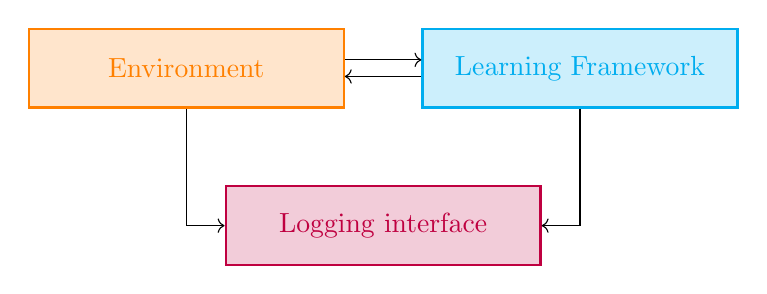
\begin{tikzpicture}
        \node[rectangle, 
        draw, 
        thick,
        minimum width = 4cm,
        minimum height = 1cm,
        color=orange,
        fill=orange!20,
        ] (A) at (0,0)  {Environment};
        \node[rectangle, 
        draw, 
        thick,
        minimum width = 4cm,
        minimum height = 1cm,
        color=cyan,
        fill=cyan!20,
        ] (B) at (5,0)  {Learning Framework};
        \node[rectangle, 
        draw, 
        thick,
        minimum width = 4cm,
        minimum height = 1cm,
        color=purple,
        fill=purple!20,
        ] (C) at (2.5,-2)  {Logging interface};

        \draw[->] ([yshift=3]A.east) -- ([yshift=3]B.west);
        \draw[<-] ([yshift=-3]A.east) -- ([yshift=-3]B.west);
        \draw[->] (B.south) |- (C.east);
        \draw[->] (A.south) |- (C.west);

        
    \end{tikzpicture}
\end{figure}

Each of these should interact for a successful implementation of the first stage.
After the environment is imported, the learning framework is imported, this is a framework used to train the agent.
Two main implementations were explored in this stage, Keras-rl and a manual implementation of the Keras API.

    \subsection*{Keras-rl}
    To implement keras-rl\cite{kerasrl2} in the specific hardware used in this project, it was required to be installed from source inside a miniforge environment.
    To be able to set up the model used by Keras-rl, TensorFlow was required. Once again, the hardware required a custom installation, the instructions can be found on the manufactures website \cite{apple-tf}.

    As the requirements were met, the next step is to setup a model, this was setup using keras, imported from TensorFlow.
\begin{figure}[H]
    \centering
    \includegraphics[width=1\textwidth]{cartpole_neural_network.eps}
    \caption{Visual representation of the neural network used to solve the CartPole Environment. }
    \label{fig:cartpole_neural_network}
\end{figure}
An implementation of the neural network used for the CartPole environment, using the structure demonstrated above is shown in the code snippet below.

\lstset{language=Python}
\lstset{frame=lines}
\lstset{caption={Setting up the model in the CartPole environment}}
\lstset{label={lst:code_direct}}
\lstset{basicstyle=\footnotesize}
\begin{lstlisting}
from tensorflow.keras.models import Sequential
from tensorflow.keras.layers import Dense, Input

states = env.observation_space.shape
actions = env.action_space.n

def build_model(states, actions):
model = Sequential() 
model.add(Input(states))
model.add(Dense(12, activation='relu', input_shape=(1,4)))
model.add(Dense(12, activation='relu'))
model.add(Dense(actions, activation='linear'))
return model

model = build_model(states, actions)
model.build(states)
\end{lstlisting}
    
    The code displayed above is used to import the required packages for the model, proceeded by a function where the model is defined. Here, we can see that the model receives the inputs and it connect to a fully-connected (Dense) layer with 12 neurons and relu activation function,
    this layer is followed by another fully connected layer with 12 neurons and relu activation function.
    
    The next step in setting up the learning framework is to define the agent. To do this, Keras-rl needs to be imported.
    
\lstset{language=Python}
\lstset{frame=lines}
\lstset{caption={Setting up the learning agent}}
\lstset{basicstyle=\footnotesize}
\begin{lstlisting}
from rl.agents import DQNAgent
from rl.policy import EpsGreedyQPolicy
from rl.memory import SequentialMemory          
from tensorflow.keras.optimizers import Adam

def build_agent(model, actions):
    policy = EpsGreedyQPolicy(eps=.3)
    memory = SequentialMemory(limit=50000, window_length=1)
    dqn = DQNAgent(model=model, memory=memory, 
    policy=policy, nb_actions=actions, 
    nb_steps_warmup=100, target_model_update=1e-2)
    return dqn

dqn = build_agent(model, actions)
dqn.compile(Adam(learning_rate=0.01), metrics=["mae"])

dqn.fit(env, nb_steps=50000)
\end{lstlisting}

In the code above, the agent, exploration policy and memory are imported from the Keras-rl library and the Adam optimizer is imported from Keras.

The $build\_agent$ function is used to set the DQNAgent, the exploration policy is initiated and $\epsilon$ value is set to 0.3.
The memory, replay buffer, is initiated using the SequentialMemory class from Keras-rl, the memory length is set to 50000 samples and the window length is set to the number of samples at each time, in this case 1.
The agent is then compiled using the Adam optimizer, where the learning rate is set to the optimal value of 0.01, here the metric use is also set to the mean absolute error.
The DQNAgent is now initiated using the model, policy and memory previously defined, along with this, the number of actions is passed as a parameter, the number of warmup steps used to avoid oscillating parameters and the target model update is set to 1e-2, this indicates how the target model is updated based on the model being trained.

The last line is used to train the agent, the environment is passed as a parameter and the number of steps is set to 50000.

\subsection*{Manual Agent implementation}
During the CartPole stage, another implementation was tested against Keras-rl, this was a manual implementation of the agent.
An agent can be split into multiple parts:
\begin{itemize}
    \item Replay buffer
    \item Action selection
    \item Target-q model update
    \item Training
\end{itemize}

The \textbf{replay buffer} is used to store the following sets of data (state, action, reward, state', done), than this is sampled in batches, this batches are used to train the neural network, the replay buffer is implemented to allow learning multiple times from the same actions and it also helps to break correlations.
\lstset{language=Python}
\lstset{frame=lines}
\lstset{caption={The following function is used to store the sets of data in the replay buffer}}
\lstset{basicstyle=\footnotesize}
\begin{lstlisting}
def remember(self, state, action, reward, next_state, done):
    item = (state, action, reward, next_state, done)
    self.memory.append(item)
\end{lstlisting}


\lstset{language=Python}
\lstset{frame=lines}
\lstset{caption={The following function is used to replay actions from the buffer and train the neural network using this}}
\lstset{basicstyle=\footnotesize}
\begin{lstlisting}
def replay(self, batch_size):
    batch = random.sample(self.memory, batch_size)
    state_batch, target_batch = [], []

    for state, action, reward, next_state, done in batch:
        target = self.get_target_q_value(state)
        if done:
            target[0][action] = reward
        else:
            Q_future = max(
                self.get_target_q_value.predict(next_state)[0])

            target[0][action] = reward + Q_future * 0.9
        state_batch.append(state)
        target_batch.append(target)
    self.q_model.fit(state_batch,
                    target_batch,
                    batch_size=batch_size,
                    verbose=0,
                    epochs=1,
                    callbacks=WandbCallback())
\end{lstlisting}

In the replay function, the buffer is sampled, and the sample obtained from the buffer contains a batch of states, actions, rewards, next states and done values.
These samples are iterated and the target values are predicted based on the state using the target model.
If the state sample is done, the calculated target q-value for the action used at the current state is set to the reward value obtained. If the simulation is not done, the target q-value for the action used is set to the reward value plus the q-value for the future state is multiplied by $\gamma$ which is set to 0.9.

The \textbf{action selection} in the manual implementation is applied as follows:

\lstset{language=Python}
\lstset{frame=lines}
\lstset{caption={The following function is used to balance exploration and exploitation to select an action}}
\lstset{basicstyle=\footnotesize}
\begin{lstlisting}
def act(self, state):
    if np.random.rand() < self.epsilon:
        return self.action_space.sample()
    q_values = self.q_model.predict(state)
    action = np.argmax(q_values[0])
    return action
\end{lstlisting}

The action selection process implemented above is based on the epsilon greedy exploration strategy, to achieve a balance between exploration and exploitation an $\epsilon$. To select an action, a random number between [0,1] is generated and compared to $\epsilon$, if the random number is smaller than $\epsilon$ a random action is sampled from the environment, this is called exploration. If the random number is higher than $\epsilon$, the model is used to predict the q-value for each action, the highest q-value is selected using the NumPy function argmax, which returns the index of the higher q-value(and therefore the best-predicted action) instead of its value.

It is important to \textbf{update the target-q model} to improve the quality of the future predictions. To do this, the target model should be updated at a set number of iterations.

\lstset{language=Python}
\lstset{frame=lines}
\lstset{caption={The following function is used to update the target-q model}}
\lstset{basicstyle=\footnotesize}
\begin{lstlisting}
def update_weights(self):
    self.target_q_model.set_weights(self.q_model.get_weights())

if self.replay_counter % 10 == 0:
    self.update_weights()
\end{lstlisting}

In the CartPole implementation, the target-q model is updated every ten times the regular model is updated,
the target-q model is updated by setting its weights to the current regular model.

The last implementation step is the \textbf{training}, as can be seen in the code bellow:

\lstset{language=Python}
\lstset{frame=lines}
\lstset{caption={The following function is used to update the target-q model}}
\lstset{basicstyle=\footnotesize}
\begin{lstlisting}
nr_episodes = 200
for episode in range(nr_episodes):
    state = env.reset()
    done = False
    total_reward = 0
    step_count = 0
    while not done:
        action = agent.act(state)
        next_state, reward, done, _ = env.step(action)
        agent.remember(state, action, reward, next_state, done)
        state = next_state
        total_reward += reward
        step_count += 1
    if len(agent.memory) >= batch_size:
        agent.replay(batch_size)
\end{lstlisting}

The code above starts by setting the number of episodes to train for, followed by the for loop, iterating for the number of set episodes over the training code.

The episode starts by resetting the environment, which returns the state of the world. When each episode starts the total reward, done state and step counter are reset.

The while loop repeats until done is set to True, ending the episode. This can be either due to the pole falling, the cart moving out of the window limits or reaching 500 steps.

At each step, an action is selected using the act function shown before, which is inside a class Agent. After selecting an action a step is performed in the environment by passing the selected action,
the environment step returns the state is transitioned to, the reward obtained, whether the episode has finished and a dictionary with extra information which, in the CartPole environment, is not set to return anything.

After each step, the information retrieved is added to the buffer and the environment state is set to the state it has transitioned to, followed by incrementing the step counter.

At the end of each episode if the number of samples in the environment is higher than the batch size required the agent samples the buffer and updates the model.


\subsection*{Weights \& Biases - WandB logging platform}
To implement the logging and enable reproducibility the platform WandB - Weights \& Biases was used, this platform has integrations with all the major machine learning tools, including Keras, TensorFlow, PyTorch, Lightning, Hugging Face, Fast.ai, Scikit and XGBoost.\cite{wandb}

WandB allows to both host the platform locally or use the free wandb cloud-based version. In order to be free from relying on external services, a self-hosted version was set up on the same machine used to run the training.
To set up the self-hosted version, docker is required as the platform is dockerized, WandB can be installed using the pip command:

\begin{center}
\$ pip install wandb 

\$ wandb login
\end{center}

To log data to wandb a project needs to be created:

\lstset{language=Python}
\lstset{frame=lines}
\lstset{caption={Code used to create a wandb project and setup logging }}
\lstset{basicstyle=\footnotesize}
\begin{lstlisting}
import wandb
from rl.callbacks import WandbLogger
run = wandb.init(
config={
    "gamma": 0.9, 
    "epsilon": 0.3,
    "target_reward": 500.0,
    "batch_size": 64,
    "win_trials": 100,
    "units": 12,
    "learning_rate": 0.01
    "metrics": "mae"
    },
project="cartpole",id="run_1")

dqn.fit(env, nb_steps=50000, callbacks=[WandbLogger()])
\end{lstlisting}

After importing the wandb package when using Keras-rl we can import a pre-built callback, WandbLogger.

By calling the wandb.init function, there are three parameters passed, config, project and id.

The project parameter is the name of the WandB project, all the runs using this project name will be grouped in the interface, allowing them to be compared. 

The second parameter is the id, corresponding to the run id, the name we want to attribute to the current session. 

The config parameter is a dictionary containing any hyperparameters and values transversal across a session that we want to log. Logging the parameters this way allows us to correlate the results to the hyperparameters and reproduce the results.

After initiating the session we can log data using pre-built callbacks built into Keras and Keras-rl.

Apart from the data being logged, it was necessary to log other data and artifacts.

\lstset{language=Python}
\lstset{frame=lines}
\lstset{caption={Logging data and artifacts to WandB}}
\lstset{basicstyle=\footnotesize}
\begin{lstlisting}
run.log(
    {"video": wandb.Video(filename, fps=30, format="mp4")})

    run.log({
    "reward":total_reward,
    "epsilon":agent.epsilon,
    "average reward":np.average(reward_history),
    "mean score":mean_score,
    "minimum reward":np.min(reward_history),
    "max reward":np.max(reward_history),
    })
\end{lstlisting}

As can be seen above it is possible to log both files, and data manually, in the first example we can see how a rendered video is logged to wandb, this is helpful as it allows to observe the progress of the training.

The second example shows how additional metrics can be logged.

\begin{figure}[H]
    \centering
    \includegraphics[width=1\textwidth]{figures/wandb.png}
    \caption{Logging data and artifacts to WandB}
\end{figure}

\section{2D Walker}
Implementing the 2D walker environment has one major difference from the CartPole, as this requires the development of a custom 2D simulation and Gym environment. After research, the tools chosen for the simulation development were Pymunk\cite{pymunk}, a python implementation of Chipmunk\cite{chipmunk}, and Pygame\cite{pygame} as the latter is integrated into pymunk, allowing for a smoother implementation of the rendering avoiding duplicate code. Once an element is implemented in pymunk, it can be directly simulated in pygame.

% how should I explain the development of the simulation ???

After the simulation was developed, the next step was to implement it in a Gym environment.
The first step is to define the observation space and action space.
As defined in the Design chapter, the robot has 8 joints each with 20 degrees of freedom and each joint can perform one of three actions(decrease, maintain and increase the angle):
    \lstset{language=Python}
    \lstset{frame=lines}
    \lstset{caption={Import necessary Gym modules and initiate action space and observation space}}
\lstset{basicstyle=\footnotesize}
\begin{lstlisting}
from gym.spaces import MultiDiscrete, Box

self.action_space = MultiDiscrete([3]*8)
self.observation_space = Box(-20,20,[8])
\end{lstlisting}

Each joint has three distinct possible actions, which can be described using a Discrete space, although, as there are eight distinct joints, the resulting actions space is [3]*8, which can be defined by using a MultiDiscrete space, a space that allows for multiple discrete action spaces.

The observation space can be defined as a continuous observation as it can take any value in the range of [-20,20] therefore it requires a Box space, used to define continuous values in Gym environments. The Box space takes as arguments the lower bound, the higher bound and shape, hence the [8], as there is an observation for each of the eight joints.

There are three main functions in a Gym environment: \textbf{step}, \textbf{reset} and \textbf{render}:

\lstset{language=Python}
\lstset{frame=lines}
\lstset{caption={Defining the step function}}
\lstset{label={lst:step}}
\lstset{basicstyle=\footnotesize}
\begin{lstlisting}
def step(self, actions):
    actions = [(a-1)*2 for a in actions]
    self.robot.ru_motor.rate = actions[0]
    self.robot.rd_motor.rate = actions[1]
    self.robot.lu_motor.rate = actions[2]
    self.robot.ld_motor.rate = actions[3]
    self.robot.la_motor.rate = actions[4]
    self.robot.ra_motor.rate = actions[5]
    self.robot.lf_motor.rate = actions[6]
    self.robot.rf_motor.rate = actions[7]

    self.robot.update()
    self.space.step(1/50)

    done = False
    reward = self.calculate_reward()

    if self.check_fall():
        done = True
        reward = -10 
    if self.check_complete(): 
        done = True  
        reward = 10

    info = {}
    observation = self.robot.get_data()

    self.last_horizontal_pos = self.robot.body.position[0]
    self.last_vertical_pos = self.robot.body.position[1]

    return(
    observation,
    reward,
    done,
    info)

\end{lstlisting}

The step function receives the action array containing the action selected for each of the joints.
The first step is to convert the action to the correct form to be applied to the motors. To do this, the action is subtracted by 1 to transform the range from [0,2] to [-1,1] this are then multiplied by the rate of the motor (2).

With the correct motor rates, this is applied to the robot motors, although this will not take an effect before the robot is updated and the space takes a step.
The robot step is set to take 50 actions per second, defined by the value passed in the step function.

After the action is executed the reward is calculated using a separate function, defined as follows:


\lstset{caption={Defining the reward function}}
\lstset{label={lst:reward}}
\begin{lstlisting}
def calculate_reward(self):
    shape = self.space.shapes[-2]
    contact_lf = len(self.robot.lf_shape.shapes_collide(b=shape).points)
    contact_rf = len(self.robot.rf_shape.shapes_collide(b=shape).points)
    if (self.robot.body.position[0] - self.last_horizontal_pos) > 1:
        reward = 1
    elif 1 > (self.robot.body.position[0] - self.last_horizontal_pos) > -1:
        reward = -1
    elif (self.robot.body.position[0] - self.last_horizontal_pos) < -1:
        reward = - 2
    if not contact_lf and not contact_rf:
            reward -= 2
    return reward
\end{lstlisting}

The reward is calculated based on the current robot's horizontal position compared to the previous position.
If the robot moves forward, it is awarded 1 point. If it stays in the same position, it is penalized with -1 point. If the robot moves backwards, it is penalized with -2 points. The reward is deducted 2 points if both feet lose contact with the ground.

Referring back to Listing \ref{lst:step} after the reward is calculated the step function checks if the robot has fallen using the following function:
\lstset{caption={Defining the function to check if the robot has fallen}}
\begin{lstlisting}
def check_fall(self):
    robot_xpos = self.robot.body.position[0]
    if self.robot.body.position[1] < self.initial_height-50:
            return True
    if robot_xpos < 0 or robot_xpos > screen_width:
            return True
    return False
\end{lstlisting}

If the robot's vertical position is lower than the initial vertical position minus a threshold (50), the robot is considered to have fallen.
If the robot's horizontal position goes outside the screen width, the robot is also considered to have fallen. The result returned by the check\_fall function is 
used to set the done variable and set the reward to -10 points in case the robot falls.

The next function call is check\_complete this checks if the robot has achieved the horizontal target position defined.
If the robot reaches the target, the episode ends and the reward is set to 10 points.

After calculating the reward and checking if the episode has ended new observation data is obtained from the environment by reading the joint's position.
Followed by updating the variable holding the last horizontal position.

The reset function in the Gym environment is used to reset the environment and simulation when a new episode starts and returns an observation.

\lstset{caption={Defining the reset function}}
\begin{lstlisting}
def reset(self):
    self.space = pymunk.Space()
    self.space.gravity = (0.0, -990)
    self.robot = Robot(self.space)
    self.robot.add_land(self.space)
    self.initial_height = self.robot.body.position[1]
    observation = self.robot.get_data()
    return(observation)
\end{lstlisting}

The reset function starts by resetting the physics engine space by initiating a new one, followed by setting the gravity applied to the objects. The next step is to re-create the robot in the space followed by the land.
The initial\_height is set and a new observation is obtained.

To allow us to visualize the environment a render function has been implemented:

\lstset{caption={Defining the render function}}
\begin{lstlisting}
def render(self, mode='human', close=False):
    if self.viewer is None:
        self.viewer = pygame.init()
        pygame_util.positive_y_is_up = True
        self.clock = pygame.time.Clock()
        self.screen = pygame.display.set_mode((screen_width, screen_height))
    self.draw_options = pygame_util.DrawOptions(self.screen)
    self.screen.fill((255, 255, 255))
    self.space.debug_draw(self.draw_options)
    pygame.display.flip()
    self.clock.tick(50)
    return pygame.surfarray.array3d(self.screen)
\end{lstlisting}

The render function starts by initiating pygame and flipping the vertical coordinates as these are inverted due to the pymunk integration. The clock and screen are initiated by passing the width and weight parameters for the screen.

After creating the screen, this is filled with white and the objects are drawn on the screen, followed by calling the flip function used to update the screen.
After updating the display the clock is ticked, the parameter passed corresponds to the maximum number of frames per second, matching the one set in pymunk.

A 3D array containing the image data is returned so that it can be displayed or added to a sequence creating a video. 

After the environment was set up, it was required to have a neural network able to support the eight simultaneous actions.

This was solved by using a neural netowrk that split into multiple independent layers for each of the joints, as exemplified bellow:

\begin{figure}[H]
    \centering
    \includegraphics[width=1\textwidth]{neural_netowrl_design}
    \caption{Neural network structure used in the 2D environment}
\end{figure}

Implementation of the neural network using the Keras API:
\lstset{caption={Implementation of the neural network using the Keras API}}
\begin{lstlisting}
def build_model():
    # Define model layers.
    units = 128
    input_layer = Input(shape=(8,))

    x = Dense(units=units, activation='relu')(input_layer)
    x = Dense(units=units, activation='relu')(x)
    x = Dense(units=units, activation='relu')(x)
    x = Dense(units=units, activation='relu')(x)
    x = Dense(units=units, activation='relu')(x)
    x = Dense(units=units, activation='relu')(x)
    x = Dense(units=units, activation='relu')(x)

    y1 = Dense(units=units, activation='relu')(x)
    y1 = Dense(units=units, activation='relu')(y1)
    y1 = Dense(units=units, activation='relu')(y1)
    y1 = Dense(units=units, activation='relu')(y1)
    y1 = Dense(units=units, activation='relu')(y1)
    y1_output = Dense(units='3', name='motor_1', activation="linear")(y1)
    y2 = Dense(units=units, activation='relu')(x)
    y2 = Dense(units=units, activation='relu')(y2)
    y2 = Dense(units=units, activation='relu')(y2)
    y2 = Dense(units=units, activation='relu')(y2)
    y2 = Dense(units=units, activation='relu')(y2)
    y2_output = Dense(units='3', name='motor_2', activation="linear")(y2)

    model = Model(inputs=input_layer,outputs=[y1_output, y2_output])

    return model

\end{lstlisting}

The code above reduces the number of outputs and therefore layers created to avoid code repetition.

One necessity noticed later during testing was how the reward was calculated during training, as the reward is calculated based on the epsilon greedy action selection it doesn't fully represent the state of the model. To fix this problem a testing function was added:
\lstset{caption={Defining the testing function}}
\begin{lstlisting}
def test_model(self):  
    rewards = []
    for _ in range(5):
        state = env.reset()
        reward_accumulater = 0
        done = False
        step_count = 0
        while not done:
            state = np.expand_dims(state,0)
            action = np.argmax(self.q_model.predict(state), axis=2).flatten()
            state, reward, done, _ = env.step(action)
            reward_accumulater += reward
            step_count += 1
            if step_count>900:
                done = True
        rewards.append(reward_accumulater)
            
    run.log({
        "test_reward_average":np.average(rewards),
        })
\end{lstlisting}

This function runs everytime the target model is updated and logs the value to WandB, allowing for a better understanding of the state of the model.
\section{3D Walker}
The initial design for the 3D environment was set to use Mujoco, a physics engine that has recently open-sourced when acquired by DeepMind.
Although, this does not allow for direct integration with ROS2 and would require developing a new control interface for the robot or a compatibility layer to link the team's control and the simulator.

Given the problems mentioned above and time constraints, using the already working simulator used by the team, Gazebo, was a better option, and therefore the decision to test Mujoco and compare its performance to Gazebo was abandoned.

To complete the 3D implementation it was necessary to develop a new Gym environment and re-purpose the learning code. 
openai\_ros is an existing ROS package that implements the OpenAI Gym environment in ROS, using the following architecture:

\begin{figure}[H]
    \centering
    \includegraphics[width=1\textwidth]{openai_ros_architecture.png}
    \caption{openai\_ros package architecture\cite{ros-gym}}
\end{figure}

Although the package was developed to be used with ROS and Bold Hearts use ROS2 and due to some incompatible dependencies, it could not be used, although a ROS2 version based on the original was developed \cite{openairos_2}. 
When trying to compile the package on the Bold Hearts ADE it failed as it required Gym and the ADE does not have the package and does not have an internet connection as the docker container is in isolation mode, to fix this problem it was necessary to enable external connections to the docker container.

\lstset{caption={Enabling external connections to the docker container}}
\begin{lstlisting}
    $ pkill docker
    $ iptables -t nat -F
    $ ifconfig docker0 down
    $ brctl delbr docker0
    $ docker -d
    $ sudo systemctl restart docker
\end{lstlisting}

After the docker container was able to connect to the internet the package was able to be compiled.

The first process to be able to control the robot was to understand all the topics and services it would require to control the simulation and the robot.

\begin{itemize}
    \item \textbf{Push commands to the joints}
\lstset{caption={Push commands to the joints}}
\begin{lstlisting}
self.node.create_publisher(
    JointCommand, 
    "/cm730/joint_commands", 
    10
)
\end{lstlisting}
    \item \textbf{Get the joint information}
\lstset{caption={Get the joint information}}
\begin{lstlisting}
self.node.create_subscription(
    JointState, 
    "/joint_states", 
    self.joint_status_callback, 
    0
)
\end{lstlisting}
    \item \textbf{Pause the simulation}
\lstset{caption={Pause the simulation}}
\begin{lstlisting}
self.node.create_client(Empty, '/pause_physics')
\end{lstlisting}
    \item \textbf{Resume the simulation}
\lstset{caption={Resume the simulation}}
\begin{lstlisting}
self.node.create_client(Empty, '/unpause_physics')
\end{lstlisting}
    \item \textbf{Reset the simulation}
\lstset{caption={Reset the simulation}}
\begin{lstlisting}
self.node.create_client(Empty, '/reset_simulation')
\end{lstlisting}
\end{itemize}

With the main controls defined, a proof of concept implementation was put in place by simplifying the architecture and ignoring the robot environment and task environment, concentrating only the basic required code into an environment file and a separate file would initiate the environment, sample random actions and push them to the robot.

The proof of concept was successful and the robot would perform the published random movements. The next step is now to develop the code into the defined architecture, this allows for an abstraction of the robot, environment and task. This architecture is important to avoid code duplication and allows the team just to define a new task when new challenges arise.



 % changed from results to experiments to be more vague and that i can explore more the process and decisions

\section{Cartpole Outcomes}
The first task developed was the classic cartpole environment,
this was helpfull in understanding core concepts of reinforcement learning and neural networks, along with it,
cartpole was essential in testing and setting up the logging interface as well as testing different implementations of the learning algorithm 
\subsection*{Keras-rl}
Keras-rl is a community maintained high level implementation of keras agents for reinforcement learning, this was the first implementaiton tested. 



The implementation of keras-rl is very easy and diesn't require a deep understanding of reinforcement learning and the leanring structure.
\subsection*{Keras API}
The second implementaiton tested was using the plain keras API, while this provides more flexibility it also requires a much deeper understandng of how reinforcement learning works.
%%%%%%%%% INSERT DETAILS HERE %%%%%%%%%
The implementaiton using the Keras API was essential to develop a necessary knowledge for the project and to progress to the next stage.
\subsection*{}

While an implementaiton using Keras-rl would be simpler and even possibly ease the itteration process, this implementation provides less flexibility and given the target of the project and 
desire to develop a deeper understanding of reinforcement learning the implementation using the Keras API was choosen to implemnt the next phases.

\subsection*{Results}

%%%%%%%%% INSERT RESULTS DATA AND ANALYSIS HERE %%%%%%%%%%%%%%%%%%

\section{2D Environment Outcomes}

\section{3D Environment Outcomes}

\section{Reward Function}


\chapter{Result Discussion}

\section{CartPole Results Discussion}
In the CartPole stage, two exploration strategies were tested, Boltzmann and Epsilon Greedy. The more popular Epsilon Greedy had the best results being able to converge to an optimal policy in half the number of steps compared to Boltzmann.

The second experiment conducted in CartPole was to find the optimal hyperparameters. As could be seen in the Results section, the optimal parameters found were learning rate of 0.01 and epsilon of 0.1. The learning rate of 0.01 tends to be a starting point for testing hyperparameters in reinforcement learning and is often the optimal value. 
The value for epsilon($\epsilon$) is the probability of choosing a random action. There needs to be a balance between exploration and exploitation. The experiment covered exploration rates starting at 10\% and tested both 20\% and 30\%, although 20\% exploration was only able to converge after 100000 steps, compared to 10\% which converged at 50000 steps. Any value tested over 20\% didn't converge in 100000 steps.

\section{2D Walker Results Discussion}

 Most of the experiments in this stage iterated over the reward function. After a lot of iterations using penalties (negative rewards) and shifting the rewards to use only positive rewards, the results became better as the walker stopped bending backwards.

 Although, over the experiments realized, when testing the q-values and their variance depending on the inputs, for the learning rate of 0.01, the q-values were very close to each other and changed very little after about 400000 steps tested when testing with a learning rate of 0.1 the q-values converged fast although the results were suboptimal. From the previous discussion we can conclude that more episodes would be necessary.
 
\chapter{Future Research}
Reinforcement learning is a very complex topic, specifically when applied to such a complex movement as robotic bipedal walking. There are many approaches to solving reinforcement learning problems. Although many areas of interest couldn't be covered, this can be explored in future research on Bipedal Robotic walking and reinforcement learning in general.

As was shown in this report, developing an optimal reward function can be complex, which is an unsolved problem in the reinforcement learning field. One promising topic suggested by the project supervisor was empowerment\cite{empowerment} by intrinsic motivations. Empowerment is a technique that aims to overcome the reward problem by equipping the robot with intrinsic rewards, using rewards such as curiosity and empowerment.

The developed project uses discrete actions although, there is a loss of information when using this method, for future research, it would be valuable to compare a policy gradient approach using continuous actions.

The initial design for this project was to use Mujoco as a physics engine. However, due to time constraints, the plan had to be changed to use Gazebo as the environment was already modelled and integrated directly with ROS2. Nonetheless, the use of Mujoco is still of interest to the team, and a comparison against Gazebo can be researched.

One of the problems when developing something as simple as a motion script for the robot is the transition to the real robot, while the script might work perfectly in the simulator, it will require adaptation to work on the real robot. This is a topic of interest for the future and understanding how, using the simulator to train most of the movement, the learning can be transferred to the real robot and how to tune the learned model when testing on the robot.



\chapter{Project Evaluation}
Walking for bipedal robots using reinforcement learning was an ambitious project. Although walking could not be achieved, this project successfully developed a working 2D walking environment with a simple humanoid, implementing OpenAI Gym with ROS2 and developing documentation and preparation for future research on the topic.

The training for this project was mainly executed using Google colab+, as incompatibilities with the computer architecture (ARM64) made training locally slower in comparison. Although, Google colab constantly crashed due to timeouts and unknown problems, making it impossible to train for extended periods of time. 
On a retrospective, it would have been a better decision to train locally as even if the training was slower, it would be able to run for very long periods of time.

As already explored, the reward function should have been tested from the beginning exclusively with positive rewards, as this would have allowed for a more efficient experiment.



Although no training was executed, the last stage was a significant achievement as it is a useful tool and development not exclusive to this project but for the team. 

\chapter{Conclusion}
Although the project's main target wasn't achieved, many objectives were successful. A 2D simulator and a 3D implementation of OpenAI Gym and ROS2 were achieved. Along with this, documentation produced shows what problems were faced and how these were mitigated, including training using Google colab, installing openai\_ros2 in the team's environment and mistakes to avoid, such as developing a reward function with a big focus on penalties. 

Starting with a simple environment such as the CartPole was good for the future of the project as it allowed for developing and testing the code in an already tested environment. It also allowed for experimentation with hyperparameters and strategies without wasting a lot of time in training. 

Developing the 2D Walker was a complex task due to the novelty of using new tools such as pymunk and pygame. Pymunk proved to be a good choice for the implementation as it is well documented, easy to use and allows for rendering directly without code duplication in pygame.

The training duration and computational power were the most limiting factors in developing this project. To achieve an optimal policy, it is clear that more and longer runs are required for testing hyperparameters and reward function variations.

A working implementation using openai\_ros2 was achieved and is ready for testing using a learning algorithm for future research.






\bibliographystyle{plain}
\bibliography{reference}
\end{document}

